\documentclass[11pt,a4paper]{article}
\usepackage{xltxtra} 
\usepackage{xgreek} 
\usepackage{amsmath}


\setmainfont[Mapping=tex-text]{CMU Serif}
\setmonofont[Mapping=tex-text]{Consolas}
\raggedbottom
\everymath{\displaystyle}
\newcommand{\HRule}{\rule{\linewidth}{0.5mm}}


\begin{document}

\begin{titlepage}
\centering

% Upper part of the page
%\includegraphics{Pyrforos.png}\\[1cm]    

\textsc{\LARGE Σχολη \\ Ηλεκτρολογων Μηχανικων \\[-3pt] και \\[6pt] Μηχανικων Υπολογιστων}\\[1.5cm]
{\Large Παράλληλα Συστήματα Επεξεργασίας}\\[0.5cm]

% Title
\HRule \\[0.5cm]
{\huge \bfseries Ενδιάμεση Αναφορά}\\[0.2cm]
\HRule \\[1.5cm]

% Authors
\begin{minipage}{0.4\textwidth}
\large
Κουτσούκος Δημήτριος \\
(ΑΜ: 03110078) \\
Χαρισόπουλος Βασίλειος \\
(ΑΜ: 03110046)
\end{minipage}

\vfill

{\large \today}
\end{titlepage}

\clearpage
\clearpage
\newpage
\section{Υλοποίηση MPI}
\subsection{Μέθοδος Jacobi}
Η επαναληπτική μέθοδος Jacobi χρησιμοποιεί τις τιμές των 4 γειτονικών σημείων του πλέγματος, οι οποίες αφορούν την προηγούμενη χρονική στιγμή του υπολογισμού. Ο τύπος της είναι
\[ u_{x,y}^{t+1} = \frac{u_{x-1,y}^t + u_{x,y-1}^t + u_{x+1, y}^t + u_{x, y+1}^t}{4} \]
Επομένως στον υπολογισμό των στοιχείων για την χρονική στιγμή $t+1$ για τυχαίο σημείο του πλέγματος δεν υπάρχουν εξαρτήσεις από άλλους υπολογισμούς που μπορεί να γίνονται ταυτόχρονα για άλλο σημείο.
\subsubsection{Διαμοιρασμός πίνακα στο MPI}
Μπορούμε να διαμοιράσουμε είτε κατά στήλες/γραμμές (1D partition), είτε να χωρίσουμε τον πίνακα σε block (2D partition). Στον έτοιμο κώδικα που δίνεται από το \texttt{parlab} υλοποιείται ο δεύτερος τύπος διαμοιρασμού, με προσαύξηση μεγέθους πίνακα στην περίπτωση που δεν επιτυγχάνεται ακριβής διαμοιρασμός στοιχείων.  Οι συναρτήσεις του MPI που χρησιμοποιούνται για το διαμοιρασμό των στοιχείων του πίνακα είναι οι \texttt{MPI\_Send, MPI\_Recv}.
\subsubsection{Ανταλλαγή στοιχείων μεταξύ επεξεργαστών}
Εφόσον ακολουθήσουμε διαμέριση κατά blocks, οι επεξεργαστές πρέπει να ανταλλάσσουν στοιχεία με όλους τους γειτονικούς τους. Κάθε επεξεργαστής θα γειτνιάζει με τουλάχιστον 2 άλλους (οριακή περίπτωση οι επεξεργαστές που έχουν αναλάβει υπολογισμούς σε γωνιακά blocks του πίνακα), και κάθε τέτοια γειτνίαση θα γίνεται μέσω γραμμής ή στήλης. Για παράδειγμα ο αριστερά γειτονικός επεξεργαστής χρειάζεται για τους υπολογισμούς του την αριστερότερη στήλη του άλλου.
Η ανταλλαγή δεδομένων μπορεί να γίνεται στην αρχή της φάσης των υπολογισμών για κάθε χρονική στιγμή $t_i$. Εναλλακτικά ο κάθε επεξεργαστής μπορεί να υπολογίζει τα στοιχεία που είναι εφικτό να υπολογίσει χωρίς δεδομένα που ανήκουν σε άλλο επεξεργαστή και η ανταλλαγή δεδομένων να γίνεται μετά από αυτή τη διαδικασία. \\
Τα δεδομένα που ανταλλάσσονται, όταν στέλνονται μέσω της \texttt{MPI\_Send} αποθηκεύοναι στον MPI Buffer, απ'όπου ανακτώνται όταν καλείται η \texttt{MPI\_Recv}. Εναλλακτικά χρησιμοποιείται η \texttt{MPI\_Sendrecv} που κάνει και τις 2 λειτουργίες με μια κλήση.

\subsubsection{Έλεγχος Σύγκλισης}
Κάθε διεργασία κάνει έλεγχο σύγκλισης στα δεδομένα που έχει υπολογίσει τοπικά μέσω της \texttt{converge()}. Η converge επιστρέφει 
\begin{itemize}
	\item 0 εάν συναντήσει αποκλίνουσες τιμές (άρα αποτυχία σύγκλισης)
	\item 1 εάν διαπιστώσει σύγκλιση
\end{itemize}
Επομένως, έχοντας χωρίσει τον πίνακα $A$ σε κομμάτια $A_i, i \in \text{\#Processors} $, συνολική σύγκλιση συνεπάγεται να έχουν συγκλίνει όλα τα κομμάτια, άρα ουσιαστικά $ \min\{\text{\texttt{converge}}(A_i) \} = 1$ (το $\min()$ αντιστοιχεί στο λογικό AND για συναρτήσεις σαν την \texttt{converge()}). Έτσι, εύκολα διαπιστώνουμε ότι μπορούμε να ελέγξουμε για συνολική σύγκλιση μέσω της \texttt{MPI\_Reduce}, χρησιμοποιώντας για τελεστή τον \texttt{MPI\_MIN}. Η \texttt{MPI\_Reduce} θα υπολογίσει το αποτέλεσμα και θα το διαθέσει μόνο στην root process (π.χ. σε αυτήν με rank = 0).
Εάν το αποτέλεσμα πρέπει να γίνει διαθέσιμο σε όλες τις διεργασίες, χρησιμοποιούμε την \texttt{MPI\_Allreduce} στη θέση της.

\clearpage
\subsection{Μέθοδος Gauss-Seidel}
Η μέθοδος Gauss-Seidel δίνεται για το διδιάστατο πλέγμα από τον τύπο
\[ u_{x,y}^{t+1} = \frac{u_{x-1,y}^{t+1} + u_{x,y-1}^{t+1} + u_{x+1, y}^t + u_{x, y+1}^t}{4} \]
δηλαδή χρησιμοποιεί τις updated τιμές 2 εκ των γειτονικών στοιχείων για τους υπολογισμούς προκειμένου να επιταχύνει την σύγκλιση. 
\subsubsection{Επικοινωνία Επεξεργαστών}
Επειδή για κάθε υπολογισμό χρειαζόμαστε τόσο τρέχουσες όσο και παρελθοντικές τιμές του πλέγματος, η επικοινωνία των επεξεργαστών αλλάζει ως προς την οργάνωση και τα στοιχεία που ανταλλάσσονται. Όταν ένας επεξεργαστής επιχειρεί να υπολογίσει το δυναμικό σε τυχαίο σημείο $(x_r, y_r)$, πρέπει να έχει στη διάθεσή του τα σημεία $x_{r-1}, y_{r-1}$ της ίδιας χρονικής στιγμής. Εάν αυτά τα σημεία βρίσκονται σε γειτονικούς επεξεργαστές, ο επεξεργαστής πρέπει να τα "ζητήσει", ενώ αντίστοιχα πρέπει να στείλει τα δικά του σημεία που θα χρειαστούν σε άλλους γειτνιάζοντες επεξεργαστές. Για τα στοιχεία που χρειάζεται, υπάρχουν 3 περιπτώσεις που παρουσιάζονται σχηματικά. \\
\begin{figure}[h]
\centering
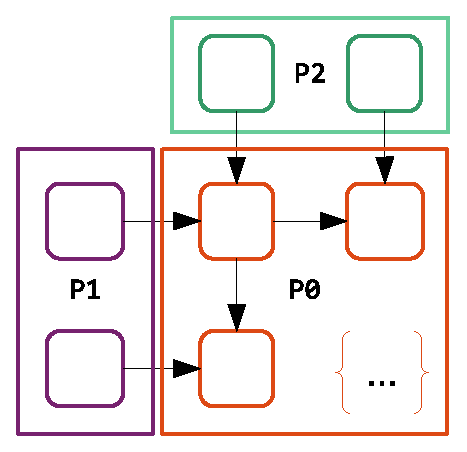
\includegraphics[scale=0.6]{gaussSeidelPull.eps}
\caption{Απαιτήσεις στοιχείων για υπολογισμό}
\end{figure}
Φαίνεται πως για τον υπολογισμό του στοιχείου στην πάνω αριστερά γωνία χρειάζονται οι ανανεωμένες τιμές από στοιχεία των επεξεργαστών \texttt{P1, P2}. Για άλλα στοιχεία του \texttt{P0} χρειάζονται οι ανανεωμένες τιμές από ένα στοιχείο εκ των επεξεργαστών \texttt{P1, P2} και ένα από \texttt{P0}. Όλα τα υπόλοιπα στοιχεία δεν χρειάζονται ανανεωμένες τιμές από άλλους επεξεργαστές. \\
Επομένως για κάθε επεξεργαστή η επικοινωνία όσον αφορά το κομμάτι των ανανεωμένων τιμών έγκειται στην ανάκτηση (recv) των τιμών της αριστερά γειτνιάζουσας στήλης και της άνω γειτνιάζουσας γραμμής των 2 γειτονικών του και την προώθηση (send) των αντίστοιχων δικών του στους κάτω και δεξιά γειτονικούς επεξεργαστές. 
\subsubsection{Ανταλλαγή δεδομένων}
Οι παρελθοντικές τιμές που χρειάζονται απο γειτνιάζοντες επεξεργαστές μπορούν να ανταλλάσσονται εξ'ολοκλήρου στην αρχή της υπολογιστικής φάσης. Για τις ανανεωμένες τιμές, προκειμένου να γίνει εφικτή η προώθηση των ανανεωμένων τιμών στους γειτονικούς επεξεργαστές πρέπει να έχει υπολογιστεί το δυναμικό σε ολόκληρο το πλέγμα λόγω της γεωμετρίας των εξαρτήσεων. Έτσι οι δυνατότητες παραλληλοποίησης είναι πολύ λιγότερες.	
\subsubsection{Ταχύτητα πυρήνα}
Λόγω της χρήσης των ανανεωμένων τιμών του πλέγματος, η ταχύτητα σύγκλισης του πυρήνα Gauss-Seidel αναμένεται να είναι καλύτερη από της Jacobi, δηλαδή θα χρειαστούν λιγότερες επαναλήψεις. Ωστόσο λόγω των data dependencies η Jacobi θα εκμεταλλεύεται καλύτερα την παραλληλία εκτέλεσης, επομένως ο χρόνος εκτέλεσης πιθανόν να είναι καλύτερος από της Gauss Seidel. 


\subsection{Μέθοδος Red-Black SOR}
Στη μέθοδο Red-Black SOR το πλέγμα χωρίζεται σε 2 σύνολα σημείων, τα κόκκινα και τα μαύρα. Το layout που προκύπτει είναι παρόμοιο με αυτό μιας σκακιέρας, δηλαδή κάθε σημείο του ενός χρώματος γειτνιάζει οριζοντίως και καθέτως με 4 σημεία του έτερου χρώματος.
Η μέθοδος περιλαμβάνει 2 διακριτές φάσεις υπολογισμού. Η πρώτη είναι η ανανέωση των "red" σημείων του πλέγματος, και δίνεται από τον τύπο
\[ u_{x,y}^{t+1} = u_{x,y}^t + \omega \frac{u_{x-1,y}^t + u_{x,y-1}^t + u_{x+1, y}^t + u_{x, y+1}^t - 4u_{x,y}^t}{4}, (x+y)\  \% \  2 == 0 \]
Παρατηρούμε ότι τα red στοιχεία υπολογίζονται μονάχα από black στοιχεία, και μάλιστα χρησιμοποιούν παρελθοντικές τιμές. Επομένως η φάση αυτή δεν περιέχει αλληλοεξαρτήσεις ή χρονικές προτεραιότητες υπολογισμών (σε αντίθεση με τη μέθοδο gauss-seidel). Η επόμενη φάση υπολογίζει τα black στοιχεία του πλέγματος για χρονική στιγμή $t+1$ με βάση την ανανεωμένη τιμή των red στοιχείων (δηλαδή για $t+1$).
\[u_{x,y}^{t+1} = u_{x,y}^t + \omega \frac{u_{x-1,y}^{t+1} + u_{x,y-1}^{t+1} + u_{x+1, y}^{t+1} + u_{x, y+1}^{t+1} - 4u_{x,y}^t}{4}, (x+y)\  \% \  2 == 1 \]
Όμως οι ανανεωμένες τιμές των red στοιχείων έχουν υπολογιστεί στην αμέσως προηγούμενη φάση και άρα είναι διαθέσιμες εξ'αρχής. Επομένως και πάλι έχουμε ευχέρεια όσον αφορά την παραλληλοποίηση της εκτέλεσης των υπολογισμών.
\end{document}

